\documentclass{llncs}

\usepackage[cp1250]{inputenc}  % or [cp1250], or [latin2], or whatever
                               % suitable for your system
\usepackage{graphicx}
\usepackage{url}

\begin{document}

\title{Connecting Web and User}

\author{Jan D�dek\inst{1} \and Alan Eckhardt\inst{2} \and Peter Vojt�\inst{2}}

\institute{Charles University, Faculty  of  Mathematics  and  Physics, Prague, Czech Republic
\and Academy of Sciences of the Czech Republic, Institute of Computer Science}

\maketitle

\begin{abstract}
The paper summarizes our research during last two years. We are concentrated on the problem of connecting web and user. This problem consists of two main aspects: user preference modelling and web content mining. We see the modelling of uncertainty beneficial to both problems and we have invested indispensable %nezanedbateln�
effort to uncertainty issues of our solutions. We see the solution of our problem (connecting web and user) in the most recent idea of web semantization, which will be also presented in this paper.
\end{abstract}

%\begin{article}

%%%%%%%%%%%%%%%%%%%%%%%%%%%%%%%%%%%%%%%%%%%%%%%%%%%%%%%%%%%%%%%%%%%%%%%%%%%%%%%%%%%%%%%%%%%%%%%%%
\section{Introduction}
%%%%%%%%%%%%%%%%%%%%%%%%%%%%%%%%%%%%%%%%%%%%%%%%%%%%%%%%%%%%%%%%%%%%%%%%%%%%%%%%%%%%%%%%%%%%%%%%%

This paper summarizes our research during last two years. We are concentrated on the problem of connecting web and user. This problem consists of two main aspects: web content mining and user preference modelling. 

Web content mining is supposed to extract structured information from possibly heterogeneous web resources. From known structure of the extracted information we can easily deduce semantics of the information and such information can be further used for precise semantic information querying. This principle is widely developed in the idea of the Semantic web. We have experimented with web content mining and exploited two different approaches: HTML structural induction and linguistic analysis. More details are presented in section~\ref{sec:webm}.

Combination of web content mining and the idea of Semantic web leaded into the formulation of the idea of gradual \emph{web semantization}, which is described in the section~\ref{sec:semantization}.

Modelling of user preferences helps user to find the most interesting information, products, offers, service, etc according to his or her preferences. Modelling of user preferences in the background of Semantic web is even more interesting and can bring useful solutions. More details about our work in this field are presented in section~\ref{sec:user}.

We see both problems (web content mining and user preference modelling) very difficult and the results are usually uncertain because they are influenced by human factor. So we see the modelling of uncertainty beneficial to both problems and we have invested indispensable %nezanedbateln�
effort to uncertainty issues of our solutions. More details are presented in section~\ref{sec:uncert}.

The whole situation is presented in the figure~\ref{img:Web2User}



\begin{figure}
\centering
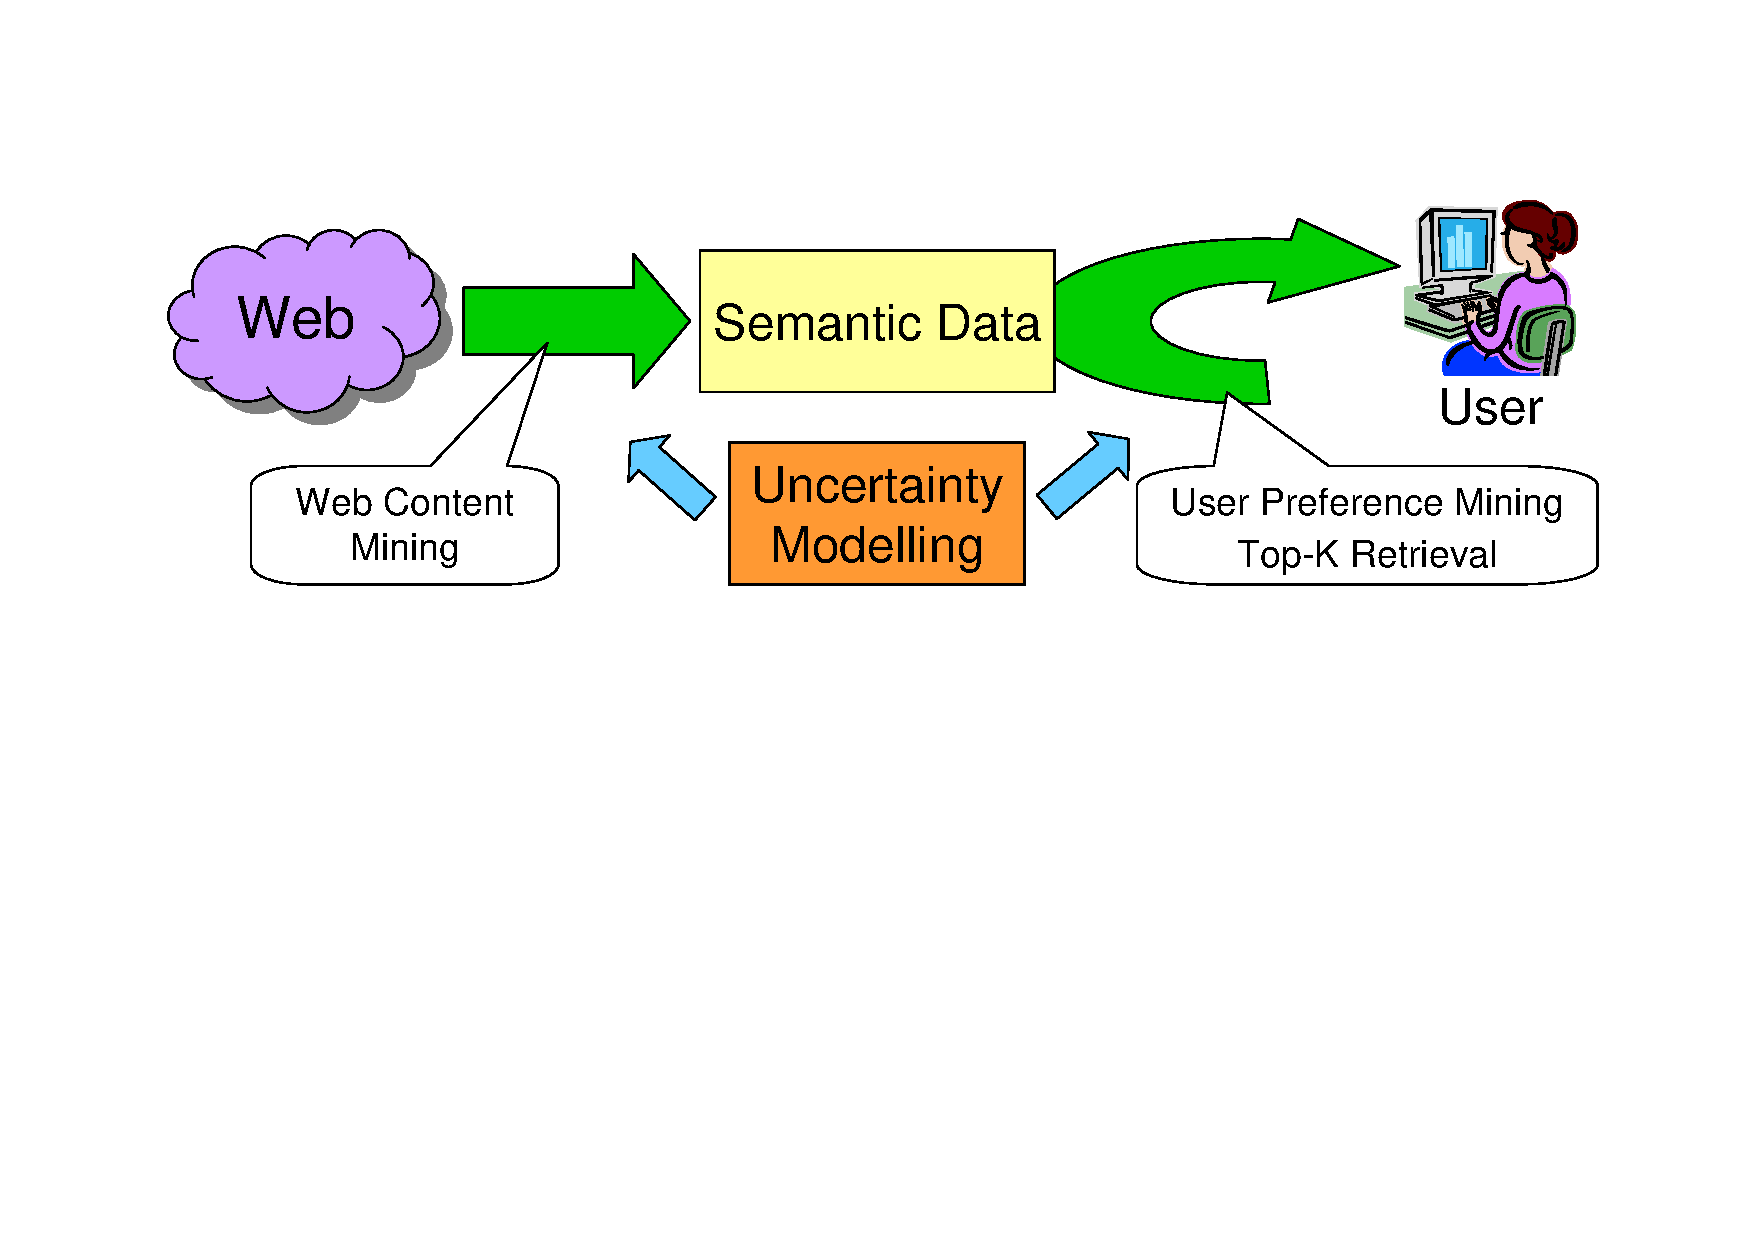
\includegraphics[width=0.9\hsize]{Web2User}
\caption{Connecting web and user.}
\label{img:Web2User}
\end{figure}


%%%%%%%%%%%%%%%%%%%%%%%%%%%%%%%%%%%%%%%%%%%%%%%%%%%%%%%%%%%%%%%%%%%%%%%%%%%%%%%%%%%%%%%%%%%%%%%%%
\section{Web Content Mining} \label{sec:webm}
%%%%%%%%%%%%%%%%%%%%%%%%%%%%%%%%%%%%%%%%%%%%%%%%%%%%%%%%%%%%%%%%%%%%%%%%%%%%%%%%%%%%%%%%%%%%%%%%%
Web content mining or web information extraction splits pages to dominantly tabular and/or textual. We will discuss our experience with both separately.

\subsection{Dominantly Tabular Pages}
In our works \cite{biblio:EcHoUncertaintyIssues2007,biblio:EcHoUncertaintyIssues2008} we have developed a software web information extraction tool that utilizes repeating structural patterns present on  ``product summary'' HTML web pages. This tool reduces human work need to extract information from such web pages. In the present this tool can be used with advantage, but is still in development and promise better results with future new features (reduction of effort connected with definition of regular expressions and exploitation of ``detail pages'' in internet shop sites). 

\subsection{Dominantly Textual Pages}
In \cite{biblio:DeVoExtrakceinformaci2008} we have introduced a linguistic-based method for extraction of information from text-based web resources in Czech. We have experimented with several linguistic tools for Czech, namely Tools for machine annotation -- PDT 2.0 and the Czech WordNet. Then in \cite{biblio:KlPrIntelligentInformation2008} we have presented a design of a system which captures text of web-pages, annotates it linguistically by PDT tools, extracts data and stores the data in an ontology. We reported on initial experiments in the domain of reports of traffic accidents. The results showed that this method can e.g. aid summarization of the number of injured people.

In \cite{biblio:DeVoLinguisticextraction2008} we focused on the data extraction phase of the system and presented methods for learning queries over linguistically annotated data. Machine learning procedure for automated learning of the linguistic queries (extraction patterns) was presented in \cite{biblio:DeEcExperimentswith2008} where we have used ILP as the learning method.
Semantic interpretation of extraction patterns and subsequent semantic interpretation of extracted data were developed in \cite{biblio:DeVoComputingaggregations2008}.

%%%%%%%%%%%%%%%%%%%%%%%%%%%%%%%%%%%%%%%%%%%%%%%%%%%%%%%%%%%%%%%%%%%%%%%%%%%%%%%%%%%%%%%%%%%%%%%%%
\section{Modelling of User Preferences} \label{sec:user}
%%%%%%%%%%%%%%%%%%%%%%%%%%%%%%%%%%%%%%%%%%%%%%%%%%%%%%%%%%%%%%%%%%%%%%%%%%%%%%%%%%%%%%%%%%%%%%%%%
User preferences became recently a hot topic. The massive use of internet shops and social webs require the presence of a user modelling, which helps users to orient themselves on a page. There are many different approaches to model user preferences. In \cite{biblio:EcInductiveModels2007} we made overview of the state-of-the-art in the area of acquisition of user preferences and their induction. Main focus was on the models of user preferences and on the induction of these models, but also the process of extracting preferences from the user behaviour was studied. We also presented our contribution to the probabilistic user models in \cite{biblio:EcInductiveModels2007}.

We focused on models of user preferences in Semantic web in \cite{biblio:EcVoUzivatelskepreference2007}. We presented a model for querying over RDF data with user preferences and for ordering of results by a user�s aggregation function. This model has theoretical base in a modification of fuzzy description logic, which is embeddable into the two valued description logic which extends OWL. We described first experiments made with Tokaf - an implementation of framework for the flexible querying.

Models of user and group preferences in social networks and the Semantic web were discussed in \cite{biblio:EcPoIntegratinguser2007}. We have constructed a model for user and group preference querying over RDF data as well as for ordering of answers by aggregation of particular attribute ranking.

In \cite{biblio:EcPoAsystem2007} we generalized Fagin�s algorithm for getting top-k answers according to user preferences. The generalization was made in two directions -- we developed some new heuristics for top-k search in the model without random access and proposed a method of ordering lists of objects by user fuzzy function. To enable different user preferences our system
does not require objects to be sorted -- instead we use a B+ tree on each of the attribute domains. This leads to a more realistic model of Web services.


Web search heuristics based on Fagin�s threshold
algorithm assume we have the user profile in the form
of particular attribute ordering and a fuzzy
aggregation function representing the user combining
function. Having these, there are sufficient algorithms
for searching top-k answers. Finding particular
attribute ordering and aggregation for a user still
remains a problem. In \cite{biblio:EcHoPHASESA2007} our main
contribution is a proof of concept of a new \emph{iterative}
process of acquisition of user preferences and attribute
ordering.



Usually different users have different fuzzy scoring function -- a user preference model. Main
goal of \cite{biblio:EcHoLearningdifferent2007} was to assign a user a preference model automatically. To achieve this we decomposed user�s fuzzy ranking function to ordering of
particular attributes and to a combination function. To solve the problem of automatic assignment of user model we design two algorithms, one for learning user preference on particular attribute and second for learning the combination function. Methods were integrated into a Fagin-like top-k querying system with some new heuristics and tested.


In connection with the development of the idea of web semantization we proposed a decomposed model: semantic search engine -- user preference agent, which was presented in \cite{biblio:EcNavrhagenta2008} and \cite{biblio:DeEcSemantickyWeb2008}. 


In \cite{biblio:EcVoConsideringdatamining2008} we deal with the problem of learning
user preferences from user�s scoring of a small sample of objects with labels from a very small linearly ordered set to use these preferences for a top-k query. We merged our terminology with economics and identified fuzzy ranking function to ordering of particular attributes as an \emph{objective function} and our combination function as an \emph{utility function}. One of the main contributions of this last work (\cite{biblio:EcVoConsideringdatamining2008}) was that we have compared our method to some classical data-mining methods. We used several measures (RMSE and rank correlations \dots) to evaluate efficiency of these methods.




%%%%%%%%%%%%%%%%%%%%%%%%%%%%%%%%%%%%%%%%%%%%%%%%%%%%%%%%%%%%%%%%%%%%%%%%%%%%%%%%%%%%%%%%%%%%%%%%%
\section{Modelling of Uncertainty} \label{sec:uncert}
%%%%%%%%%%%%%%%%%%%%%%%%%%%%%%%%%%%%%%%%%%%%%%%%%%%%%%%%%%%%%%%%%%%%%%%%%%%%%%%%%%%%%%%%%%%%%%%%%
We are interested in replacing human processing of web resources by automated processing. Based on an experimental system we identified uncertainty issues making this process difficult for automated processing and tried to minimize human intervention in \cite{biblio:EcHoUncertaintyIssues2007} and \cite{biblio:EcHoUncertaintyIssues2008}. In particular we focus on uncertainty issues in a web content mining system and a user preference mining system.

In \cite{biblio:DeEcDiscussionUncertainty2008} we discussed the what, who, when, where, why and how of uncertain reasoning based on achievements of URW3XG\footnote{\url{http://www.w3.org/2005/Incubator/urw3/XGR-urw3/}}, our experiments and some future plans.  
\begin{description}
\item[What and Why] -- improving semantic web practice through uncertain reasoning.
\item[Who and When] -- will create, maintain and use this annotation. Will this annotation be done by a human creator using an annotation supporting tool for web page creation? Or will it be done by a third party annotation? For this, we discussed a refinement of URW3XG use cases. Possible use of this enriched web will be for humans and services.
\item[Where] -- will be this annotations stored. Our proposal is based on the web crawler Egothor repository\footnote{\url{http://www.egothor.org/}} (we have crawled data in size of several TB from .cz domain) and an additional semantic repository build on the top using data pile technology \cite{biblio:BeObDataIntegration2005}. 
\item[How] -- to semantically enrich information and how to measure success and/or progress of such enrichment. This problem consists of two parts, namely, a data mining task and an ontology modelling task. Third party annotation of great size can be done only in an automated way and it should be done according to an ontology. 
\end{description}

In \cite{biblio:DeEcDiscussionUncertainty2008} and \cite{biblio:DeEcSemantickyWeb2008} our annotation ontology grew out of URW3XG uncertainty ontology and extended some features needed for annotation. We started here from an assumption that a part of annotation will be done by a web information extraction and that this is the main source of uncertainty.

Success of this approach can be measured primarily by the advance of semantic web functionalities. This is easier to measure for software agents. More difficult is to design metrics to measure human user satisfaction. All these aspects were discussed in the presentation of \cite{biblio:DeEcDiscussionUncertainty2008}.

%%%%%%%%%%%%%%%%%%%%%%%%%%%%%%%%%%%%%%%%%%%%%%%%%%%%%%%%%%%%%%%%%%%%%%%%%%%%%%%%%%%%%%%%%%%%%%%%%
\section{Web Semantization} \label{sec:semantization}
%%%%%%%%%%%%%%%%%%%%%%%%%%%%%%%%%%%%%%%%%%%%%%%%%%%%%%%%%%%%%%%%%%%%%%%%%%%%%%%%%%%%%%%%%%%%%%%%%
Nobody seems to care in the semantic web community about the content of the web of today or of pages published without annotations. By our opinion the content of the web of today is too valuable to be lost for emerging semantic web applications. The problem of \emph{semantization} (enrichment) of current web content as an automated process of third party annotation for making (at least a part, increasing in time) of today web accessible for machine processing and hence enabling intelligent tools for searching and recommending things on the web. Our main idea (presented in \cite{biblio:DeEcSemantickyWeb2008}) is to create a semantic repository of information automatically extracted from the web and corresponding annotated copies of (mainly textual) parts of web pages, and make it available to intelligent agents.


%%%%%%%%%%%%%%%%%%%%%%%%%%%%%%%%%%%%%%%%%%%%%%%%%%%%%%%%%%%%%%%%%%%%%%%%%%%%%%%%%%%%%%%%%%%%%%%%%
%\section{Conclusion}
%%%%%%%%%%%%%%%%%%%%%%%%%%%%%%%%%%%%%%%%%%%%%%%%%%%%%%%%%%%%%%%%%%%%%%%%%%%%%%%%%%%%%%%%%%%%%%%%%
%We have presented a 

\vspace{0.5cm}
\noindent\textbf{Acknowledgments}

\noindent This work was partially supported by the Ministry of Education of the Czech Republic (grant MSM0021620838) and by Czech projects 1ET100300517 and 1ET100300419.


\bibliographystyle{splncs}
\bibliography{SemWeb_1ET100300419}

%\end{article}
\end{document}

